\documentclass{beamer}

\usepackage[utf8]{inputenc}

\usepackage{alltt}
\usepackage{xcolor}
\usepackage[overlay,absolute]{textpos}
\usepackage[normalem]{ulem}

\usepackage{tikz}
\usetikzlibrary{arrows,petri,topaths}
\usepackage{tkz-berge}

%% Colors for source highlighting
\definecolor{scKW}  {HTML}{AA37F2}
\definecolor{scFct} {HTML}{1010FF}
\definecolor{scType}{HTML}{228B22}
\definecolor{scVar} {HTML}{A45936}
\definecolor{scComm}{HTML}{B32525}

%% Define _s_cala commands
\newcommand{\sK}[1]{{\color{scKW} #1}}
\newcommand{\sF}[1]{{\color{scFct} #1}}
\newcommand{\sV}[1]{{\color{scVar} #1}}
\newcommand{\sT}[1]{{\color{scType} #1}}
\newcommand{\sC}[1]{{\color{scComm} #1}}
\newcommand{\sH}[1]{{\color{white} #1}}
\newcommand{\sN}[1]{{\color{black} #1}}
\newcommand{\sS}{\vspace{0.8mm}}

%% Define other commands
\newcommand<>{\strike}[1]{\alt#2{\sout{#1}}{#1}}

\setbeamercovered{transparent}
\setbeamertemplate{navigation symbols}

\setbeamertemplate{footline}{\makebox[0.98\paperwidth][r]{\large \raisebox{1.2ex}{\insertframenumber}}}

\title{FlowPools}
\subtitle{A Lock-Free Deterministic Concurrent Dataflow Abstraction}

\author{Aleksandar Prokopec \and Heather Miller \and Tobias Schlatter
  \and Philipp Haller \and Martin Odersky}
\date{September 12, 2012}
\institute{LAMP, EPFL}

\begin{document}

\begin{frame}
  \titlepage
\end{frame}

\section{Introduction}

% \begin{frame}
%   \frametitle{Some Context \& Motivation}
  
%   \begin{columns}
%     \begin{column}{.5\textwidth}
%       \begin{itemize}
%       \item Paper in LCPC
%       \item Project Focus:\\
%         Multi-Lane FlowPools
%       \item $49 - 54\%$ speedup
%       \end{itemize}
%     \end{column}

%     \begin{column}{.5\textwidth}
%       \includegraphics[trim = 157mm 0mm 140mm 0mm, clip, width=\textwidth]
%       {../../benchmarks/pres_graphs/cpu-scaling-insert}
%     \end{column}
%   \end{columns}

% \end{frame}


\begin{frame}
  \frametitle{Outline}
  
  \begin{block}{What is a FlowPool}\end{block}
  \begin{block}{Implementation}\end{block}
  \begin{block}{Multi-Lane FlowPools}\end{block}
  \begin{block}{Benchmarks}\end{block}

\end{frame}

\section{What is a FlowPool}

\begin{frame}
  \frametitle{What is a FlowPool}
  \framesubtitle{Big Picture}

  \begin{columns}[t]
    \column{.5\textwidth}

    Pool: concurrent collections abstraction for Scala

    \begin{block}{FlowPool Properties}
      \begin{itemize}
      \item<1> Pool semantics
      \item<2,3,4> Asynchronous
      \item<5> Deterministic
      \item<6> Lock-Free
      \item<7> Unneeded Elements GC'd
      \end{itemize}
    \end{block}

    \column{.5\textwidth}

    \begin{overprint}
      \onslide<1>
      \begin{block}{Pool semantics}
        \begin{itemize}
        \item Unordered
        \item Multiple occurrences
        \item Insertion (\texttt{<<})
        \item Traversal (\texttt{foreach})
        \end{itemize}
      \end{block}

      \onslide<2>
      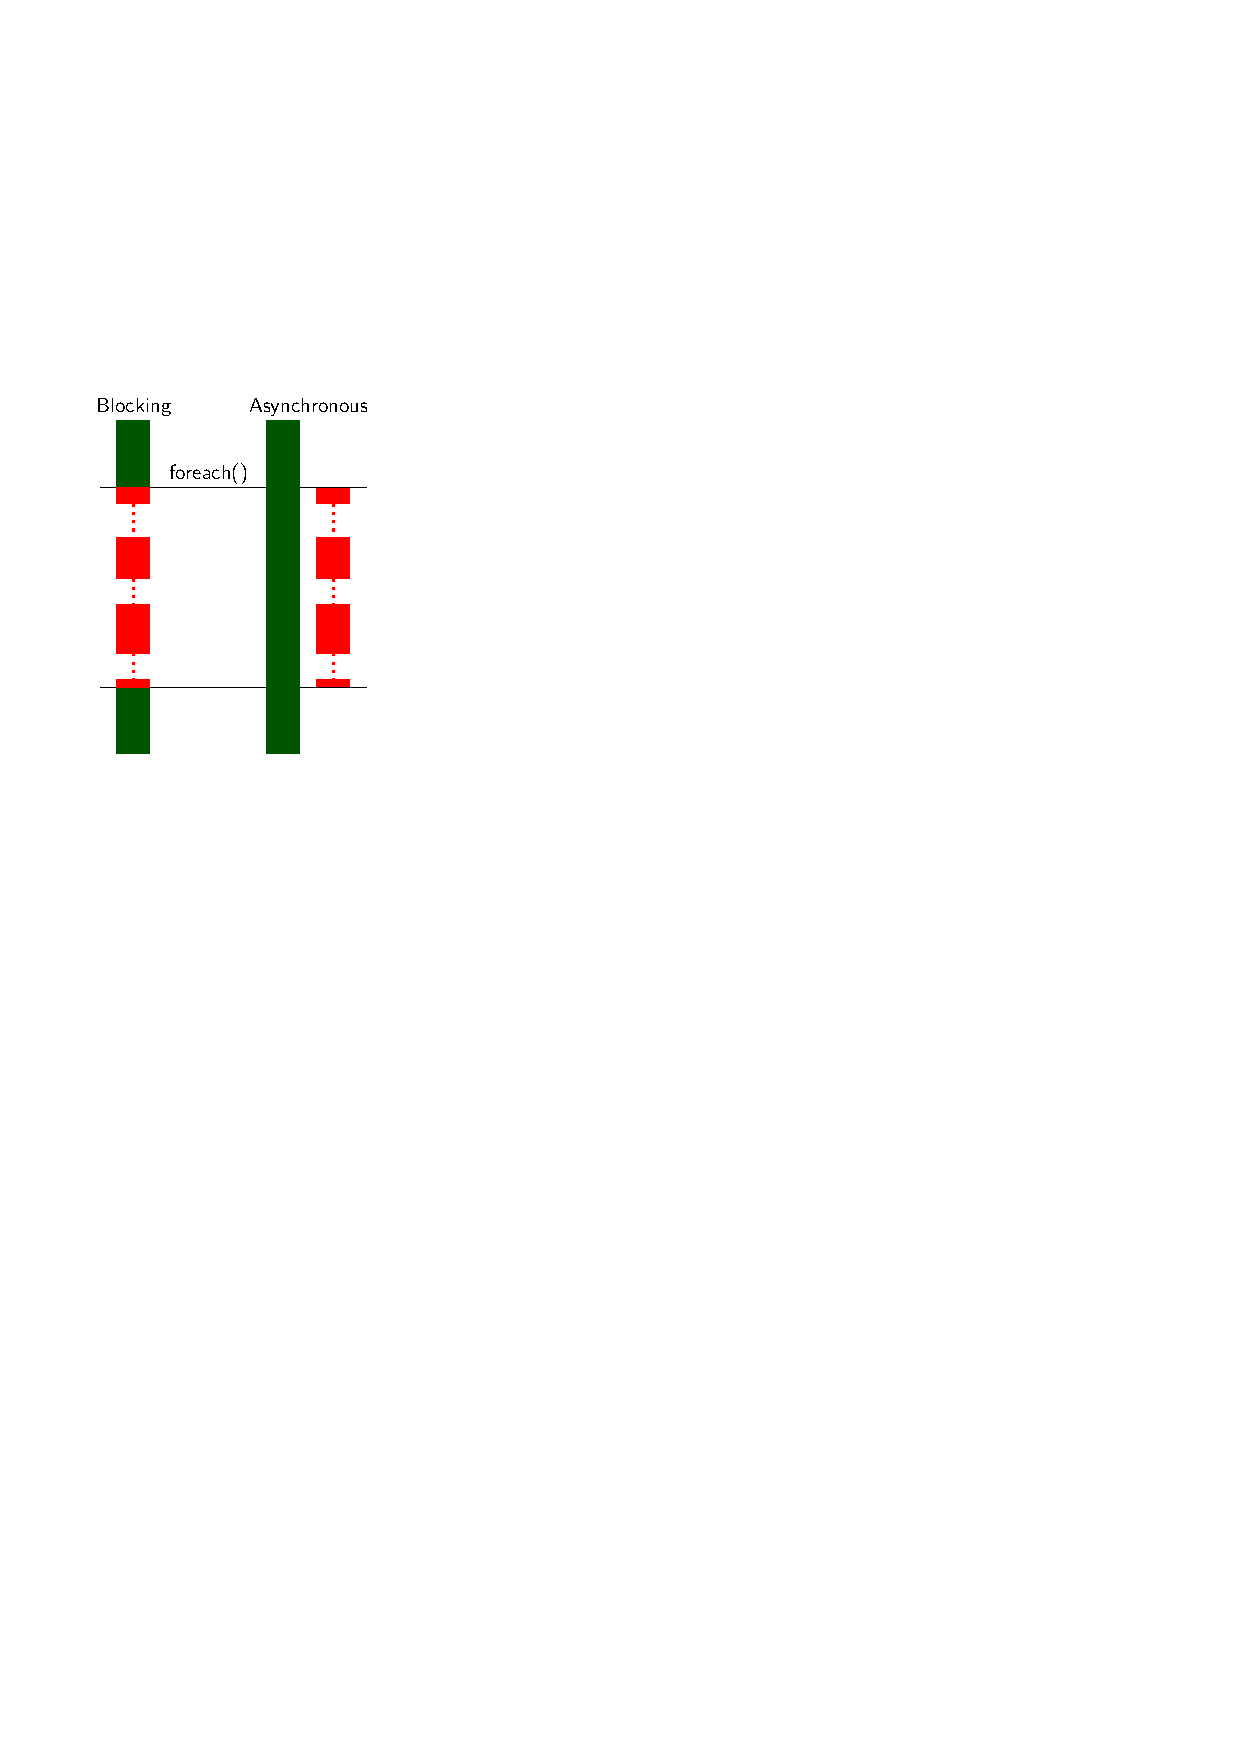
\includegraphics[page=1]{figs/async}

      \onslide<3>
      \includegraphics[page=2]{figs/async}

      \onslide<4>
      \begin{block}{Closures}
        \begin{alltt} \small
          \sK{val} \sV s = \sK{new} FlowPool[Int]\\
          \sK{val} \sV c = 5\\
          \\
          c.foreach \{\\
          \sH{\ \ }x => println(c + x)\\
          \}
        \end{alltt}
      \end{block}

      \onslide<5>
      \begin{block}{Determinism}
        Every execution of a given program with given input eventually
        \begin{itemize}
        \item Always reaches same state
        \item[] \qquad or
        \item Always fails
        \end{itemize}
      \end{block}

      \onslide<7>
      \begin{block}{Garbage Collection}
        \begin{alltt}
          \sK{def} create() = \{\\
          \sH{\ \ }\sK{val} a = \sK{new} Object()\\
          \sH{\ \ }\sK{val} b = \sK{new} Object()\\
          \sH{\ \ }\sK{return} a\\
          \}\\
          \\
          \sK{val} x = create()
        \end{alltt}
      \end{block}

    \end{overprint}

  \end{columns}

\end{frame}

\begin{frame}
  \frametitle{What is a FlowPool}
  \framesubtitle{Programming Model -- Elementary Operations}

  \begin{alltt} \small
    \sK{def} \sF{<<}(\sV x: \sT T): \sK{this}.\sK{type}\sS\\
    \strike<7>{\sK{def} \sF{foreach}[\sT U](\sV f: \sT{T => U}): \sT{Future[Unit]}}\sS\\
    \uncover<2->{\sK{def} \sF{seal}(\sV{size}: \sT{Int}): \sT{Unit}\sS}\\
    \uncover<6->{\sK{def} \sF{aggregate}[\sT S](\sV{zero}: \sT{=>S})(\sV{cmb}: \sT{(S, S) => S})}\\
    \uncover<6->{\sH{def aggregate[S]}(\sV{folder}: \sT{(S, T) => S}): \sT{Future[S]}}\\
    \sH{\ \ }
  \end{alltt}

  \begin{overprint}
    \onslide<3,4>
    \texttt{Thread 1:            \qquad \qquad \qquad Thread 2:}\\
    \texttt{\sH{\ \ }p << x\sH{\ \ } \qquad \qquad \qquad \sH{\ \ }p.seal(\only<4>{1})}
    \onslide<5>
    \begin{alltt} \small
      \sK{def} \sF{fill}[\sT T](\sV n: \sT{Int})(\sV{el}: \sT{=>T}): \sT{FlowPool[T]} = \{\\
      \sH{\ \ }\sK{val} \sV p = \sK{new} FlowPool[T]\\
      \sH{\ \ }\sK{for} (i <- 1 to n) \{ p << el \}\\
      \sH{\ \ }p.seal(n); p\\
      \}
    \end{alltt}
    \onslide<6>
    \begin{alltt} \small
      \sK{def} \sF{filter}(\sV{pred}: \sT{T => Boolean}): \sT{FlowPool[T]} = \{\\
      \sH{\ \ }\sK{val} \sV p = \sK{new} FlowPool[T]\\
      \sH{\ \ }\sK{this}.aggregate(0)(\_ + \_) \{\\
      \sH{\ \ \ \ }(acc, x) => \sK{if} pred(x) \{\\
      \sH{\ \ \ \ \ \ }p << x; acc + 1\\
      \sH{\ \ \ \ }\} \sK{else} acc\\
      \sH{\ \ }\} map \{ sz => p.seal(sz) \}; p\\
      \}
    \end{alltt}
    \onslide<7>
    \begin{alltt} \small
      \sK{def} \sF{foreach}[\sT U](\sV f: \sT{T => U}): \sT{Future[Unit]} = \{\\
      \sH{\ \ }aggregate(())((\_, \_) => ()) \{\\
      \sH{\ \ \ \ }(acc, x) => f(x); ()\\
      \sH{\ \ }\}\\
      \}
    \end{alltt}
  \end{overprint}

  \begin{textblock}{2}(13,9)
    \begin{onlyenv}<5>
      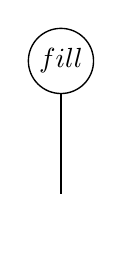
\begin{tikzpicture}[ node distance = 2cm ]
        \tikzset{EdgeStyle/.style={post}}       % directed edges
      
        \Vertex[x = 0, y = 2, L = $fill$]{S}

        \SetVertexNormal[LineColor=white] 
        \Vertex[x = 0, y = 0, L = { }]{G}
        \SetVertexNormal[LineColor=black] 

        \Edge(S)(G)

      \end{tikzpicture}  
    \end{onlyenv}
  \end{textblock}

  \begin{textblock}{2}(13,9)
    \begin{onlyenv}<6>
      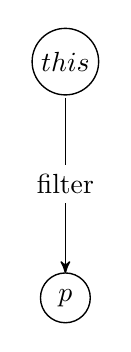
\begin{tikzpicture}[ node distance = 2cm ]
        \tikzset{EdgeStyle/.style={post}}       % directed edges
      
        \Vertex[x = 0, y = 3, L = $this$]{S}
        \Vertex[x = 0, y = 0, L = $p$]{G}

        \Edge[label = filter](S)(G)

      \end{tikzpicture}  
    \end{onlyenv}
  \end{textblock}

\end{frame}

\begin{frame}
  \frametitle{What is a FlowPool}
  \framesubtitle{Programming Model -- Higher Level Operations}

    \begin{alltt} \small
      \sK{def} \sF{foreach}[\sT U](\sV f: \sT{T => U}): \sT{Future[Unit]}\sS\\
      \sK{def} \sF{++}[\sT{S >: T}](\sV{that}: \sT{FlowPool[S]}): \sT{FlowPool[S]}\sS\\
      \sK{def} \sF{filter}(\sV p: \sT{T => Boolean}): \sT{FlowPool[T]}\sS\\
      \sK{def} \sF{map}[\sT S](\sV f: \sT{T => S}): \sT{FlowPool[S]}\sS\\
      \sK{def} \sF{flatMap}[\sT S](\sV f: \sT{T => FlowPool[S]}): \sT{FlowPool[S]}\sS\\
      \sK{def} \sF{fold}[\sT{U >: T}](\sV z: \sT U)(\sV{op}: \sT{(U, U) => U}): \sT{Future[U]}\sS\\
      \sH{\ }\\
      \sK{def} \sF{fill}[\sT T](\sV n: \sT{Int})(\sV{el}: \sT{=>T}): \sT{FlowPool[T]} \sS\\
      \sK{def} \sF{iterate}[\sT T](\sV{start}: \sT T, \sV{len}: \sT{Int})(\sV f: \sT{(T) => T}): \sT{FlowPool[T]}
    \end{alltt}

\end{frame}

\begin{frame}
  \frametitle{What is a FlowPool}
  \framesubtitle{Flow Graph}

  \begin{columns}
    \begin{column}{.5\textwidth}

      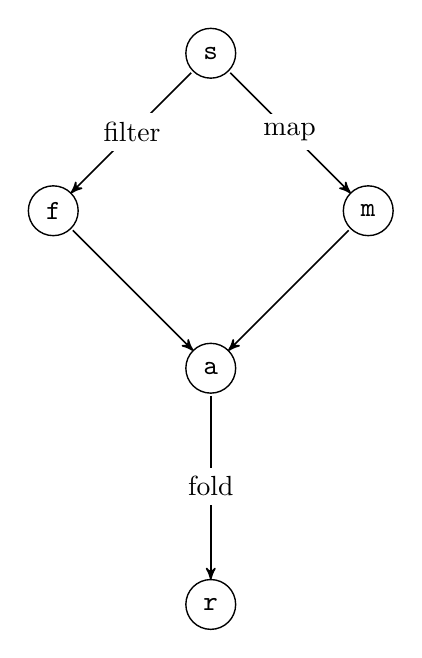
\begin{tikzpicture}[ node distance = 2cm ]
        \tikzset{EdgeStyle/.style={post}}       % directed edges

        \Vertex[x =  2, y =  7, L = \texttt{s}]{S}

        \uncover<2->{
          \Vertex[x =  4, y =  5, L = \texttt{m}]{M}
          \Edge[label = map](S)(M)
        }

        \uncover<3->{
          \Vertex[x =  0, y =  5, L = \texttt{f}]{F}
          \Edge[label = filter](S)(F)
        }

        \uncover<4->{
          \Vertex[x =  2, y =  3, L = \texttt{a}]{A}
          \Edge(M)(A)
          \Edge(F)(A)
        }

        \uncover<5->{
          \Vertex[x =  2, y =  0, L = \texttt{r}]{R}
          \Edge[label = fold](A)(R)
        }

        % \tikzset{EdgeStyle/.append style = {bend right}}

      \end{tikzpicture}  

    \end{column}

    \begin{column}{.5\textwidth}
      
      \begin{alltt}
        s = \sK{new} FlowPool[Int]\\
        \uncover<2->{m = s.map(\_ * 2)}\\
        \uncover<3->{f = s.filter(\_ > 10)}\\
        \uncover<4->{a = m ++ f}\\
        \uncover<5->{r = a.fold(0)(\_ + \_)}\\
        \sH{\ }\\
        \uncover<6->{
        s.seal(1000)\\
        \sK{for} (i <- 1 to 1000) \{\\
        \sH{\ \ }s << i\\
        \}
        }
      \end{alltt}

    \end{column}

  \end{columns}

\end{frame}

\section{Implementation}

\begin{frame}
  \frametitle{Implementation}
  \framesubtitle{Basic Structure / Garbage Collection of Unneeded Elements}

  \begin{center}
    \includegraphics<1>[page=1]{figs/SLFP}
    \includegraphics<2>[page=2]{figs/SLFP}
    \includegraphics<3>[page=3]{figs/SLFP}
    \includegraphics<4>[page=4]{figs/SLFP}
    \includegraphics<5>[page=5]{figs/SLFP}
  \end{center}

\end{frame}

\begin{frame}
  \frametitle{Implementation}
  \framesubtitle{Insert \quad \texttt{\sF{<<}\sN(\sV x\sN:\;\sT T\sN)}}

  \begin{center}
    \includegraphics<1>[page=1]{figs/SLFP_insert}
    \includegraphics<2>[page=2]{figs/SLFP_insert}
    \includegraphics<3>[page=3]{figs/SLFP_insert}
    \includegraphics<4>[page=4]{figs/SLFP_insert}
    \includegraphics<5>[page=5]{figs/SLFP_insert}
    \includegraphics<6>[page=6]{figs/SLFP_insert}
    \includegraphics<7>[page=7]{figs/SLFP_insert}
  \end{center}

  \begin{enumerate}
    \item<4-> \texttt{next = block(i+1)}
    \item<4-> \texttt{curo = block(i)}
    \item<5-> \texttt{CAS(block(i+1), next, curo)}
    \item<6-> \texttt{CAS(block(i), curo, W)}
    \item<7-> \texttt{invokeCallbacks(W, curo)}
  \end{enumerate}

\end{frame}

\begin{frame}
  \frametitle{Implementation}
  \framesubtitle{Wrong Insert \quad \texttt{\sF{<<}\sN(\sV x\sN:\;\sT T\sN)}}

  \begin{center}
    \includegraphics<1>[page=1]{figs/SLFP_wrong_insert}
    \includegraphics<2>[page=2]{figs/SLFP_wrong_insert}
    \includegraphics<3>[page=3]{figs/SLFP_wrong_insert}
    \includegraphics<4,5>[page=4]{figs/SLFP_wrong_insert}
    \includegraphics<6>[page=5]{figs/SLFP_wrong_insert}
    \includegraphics<7>[page=6]{figs/SLFP_wrong_insert}
  \end{center}

  \begin{enumerate}
  \item<1-> \texttt{curo = block(i)\phantom{xxxx}(= C)}
  \item<4-> \texttt{next = block(i+1)\phantom{xx}(= C')}
  \item<6-> \texttt{CAS(block(i+1), next, curo)}
  \item<7-> \texttt{CAS(block(i), curo, W)}
  \item<7-> \texttt{invokeCallbacks(W, curo)}
  \end{enumerate}

  % Observed State box
  \begin{textblock}{6}(9.5,8.6)  
    \begin{visibleenv}<5->
      Observed State (\alert<5>{inconsistent})
      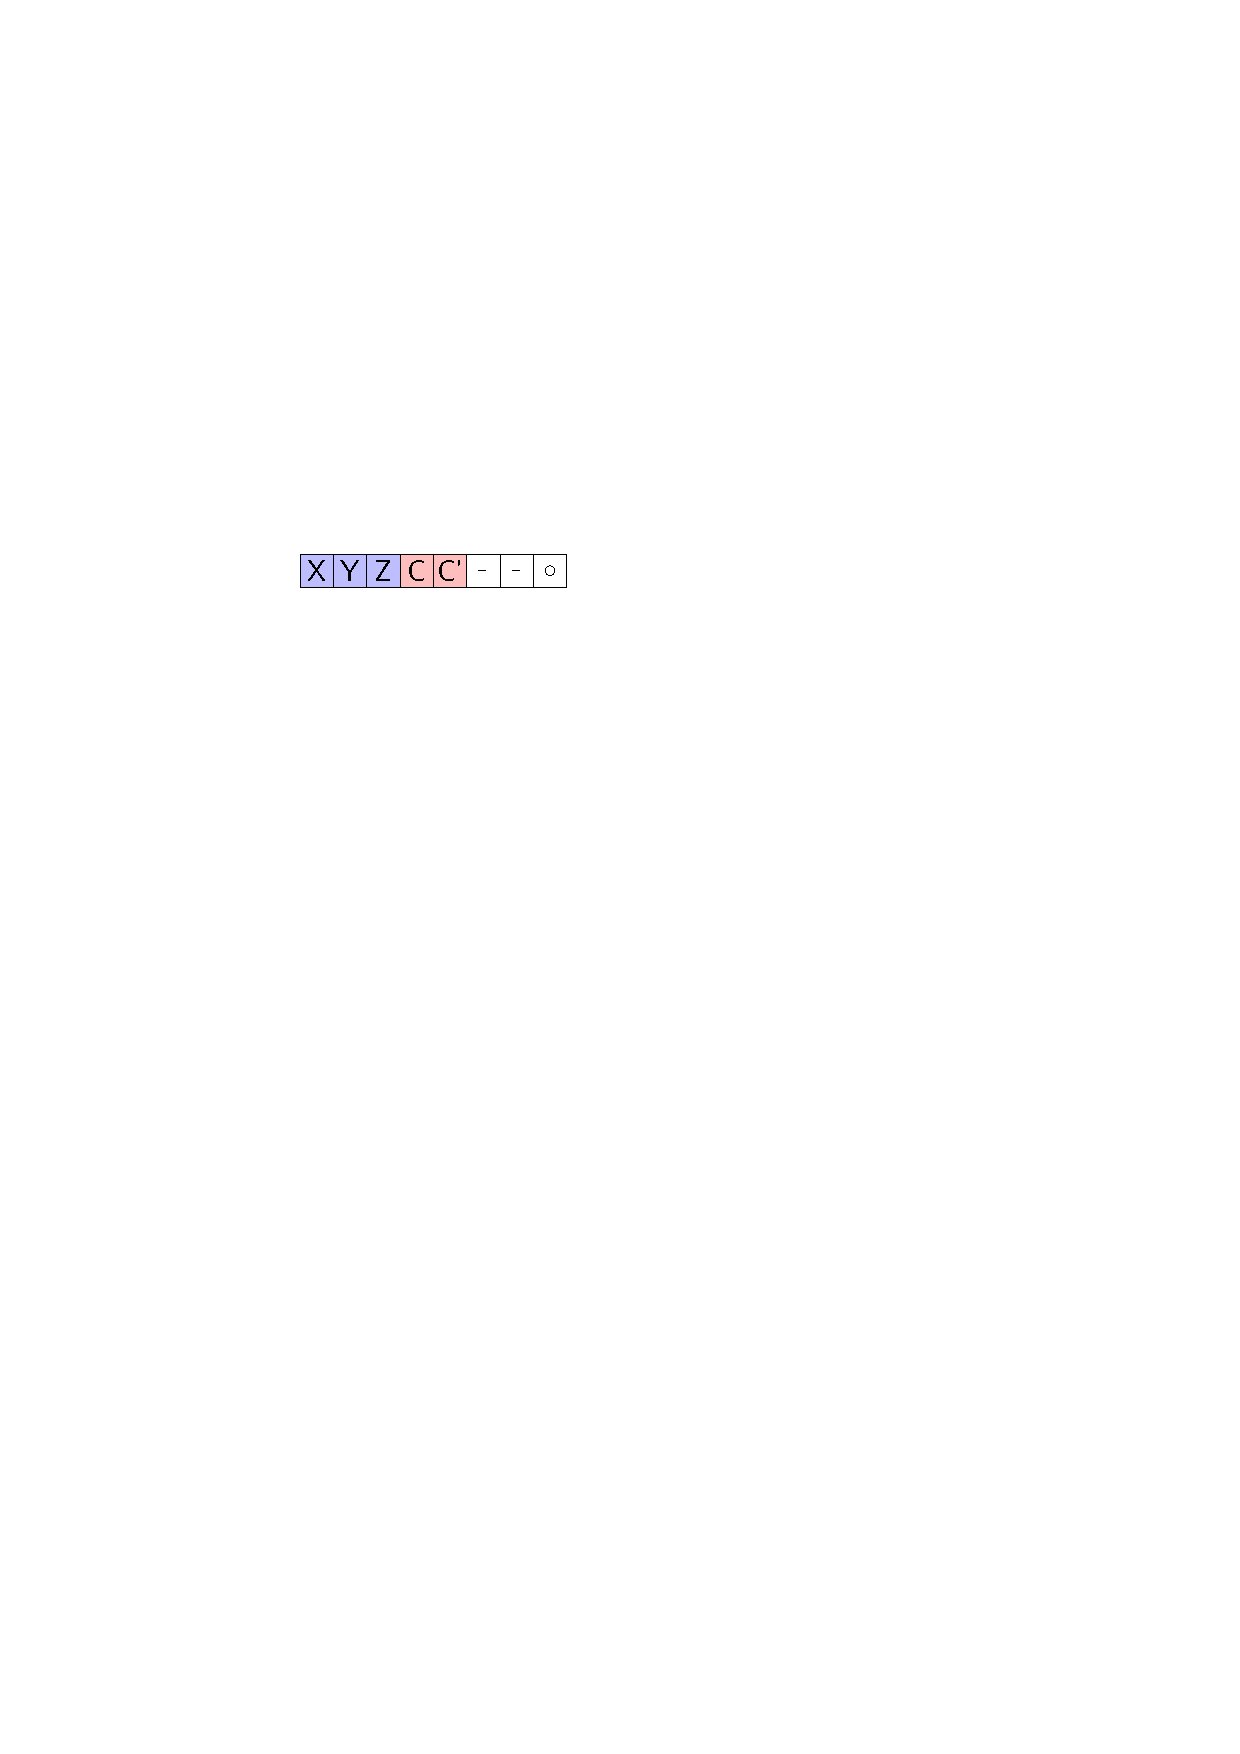
\includegraphics{figs/wrong_state}
    \end{visibleenv}
  \end{textblock}

\end{frame}

\begin{frame}
  \frametitle{Implementation}
  \framesubtitle{Seal \quad \texttt{\sF{seal}\sN(\sV n\sN:\;\sT{Int}\sN)}}

  \begin{center}
    \includegraphics<1>[page=1]{figs/SLFP_seal}
    \includegraphics<2>[page=2]{figs/SLFP_seal}
    \includegraphics<3>[page=3]{figs/SLFP_seal}
    \includegraphics<4>[page=4]{figs/SLFP_seal}
  \end{center}

  \begin{enumerate}
    \item<2-> \texttt{cbs = block(i)}
    \item[]<3-> \texttt{s = Seal(sealsize, cbs)}
    \item<4-> \texttt{CAS(block(i), cbs, s)}
  \end{enumerate}

\end{frame}

\section{Multi-Lane FlowPools}

\begin{frame}
  \frametitle{Multi-Lane FlowPools}

  \begin{block}{Single-Lane FlowPools: Issues}
    \begin{itemize}
    \item Bad scaling (insertions)
      \begin{itemize}
      \item CAS failures
      \item Cache contention
      \end{itemize}
    \end{itemize}
  \end{block}

  \pause
  \begin{block}{Solution}
    \begin{itemize}
    \item Use unordered property
    \item Extend to multiple lanes
    \item Scales nicely
    \item BUT: Seal is complex
    \end{itemize}
  \end{block}

\end{frame}


\section{Benchmarks}

\begin{frame}
  \frametitle{Benchmarks}
  \framesubtitle{CPU-Scaling -- Insertions}

  %% Hack to use whole frame
  \begin{columns}[c]
    \begin{column}{\paperwidth}
      \centering
      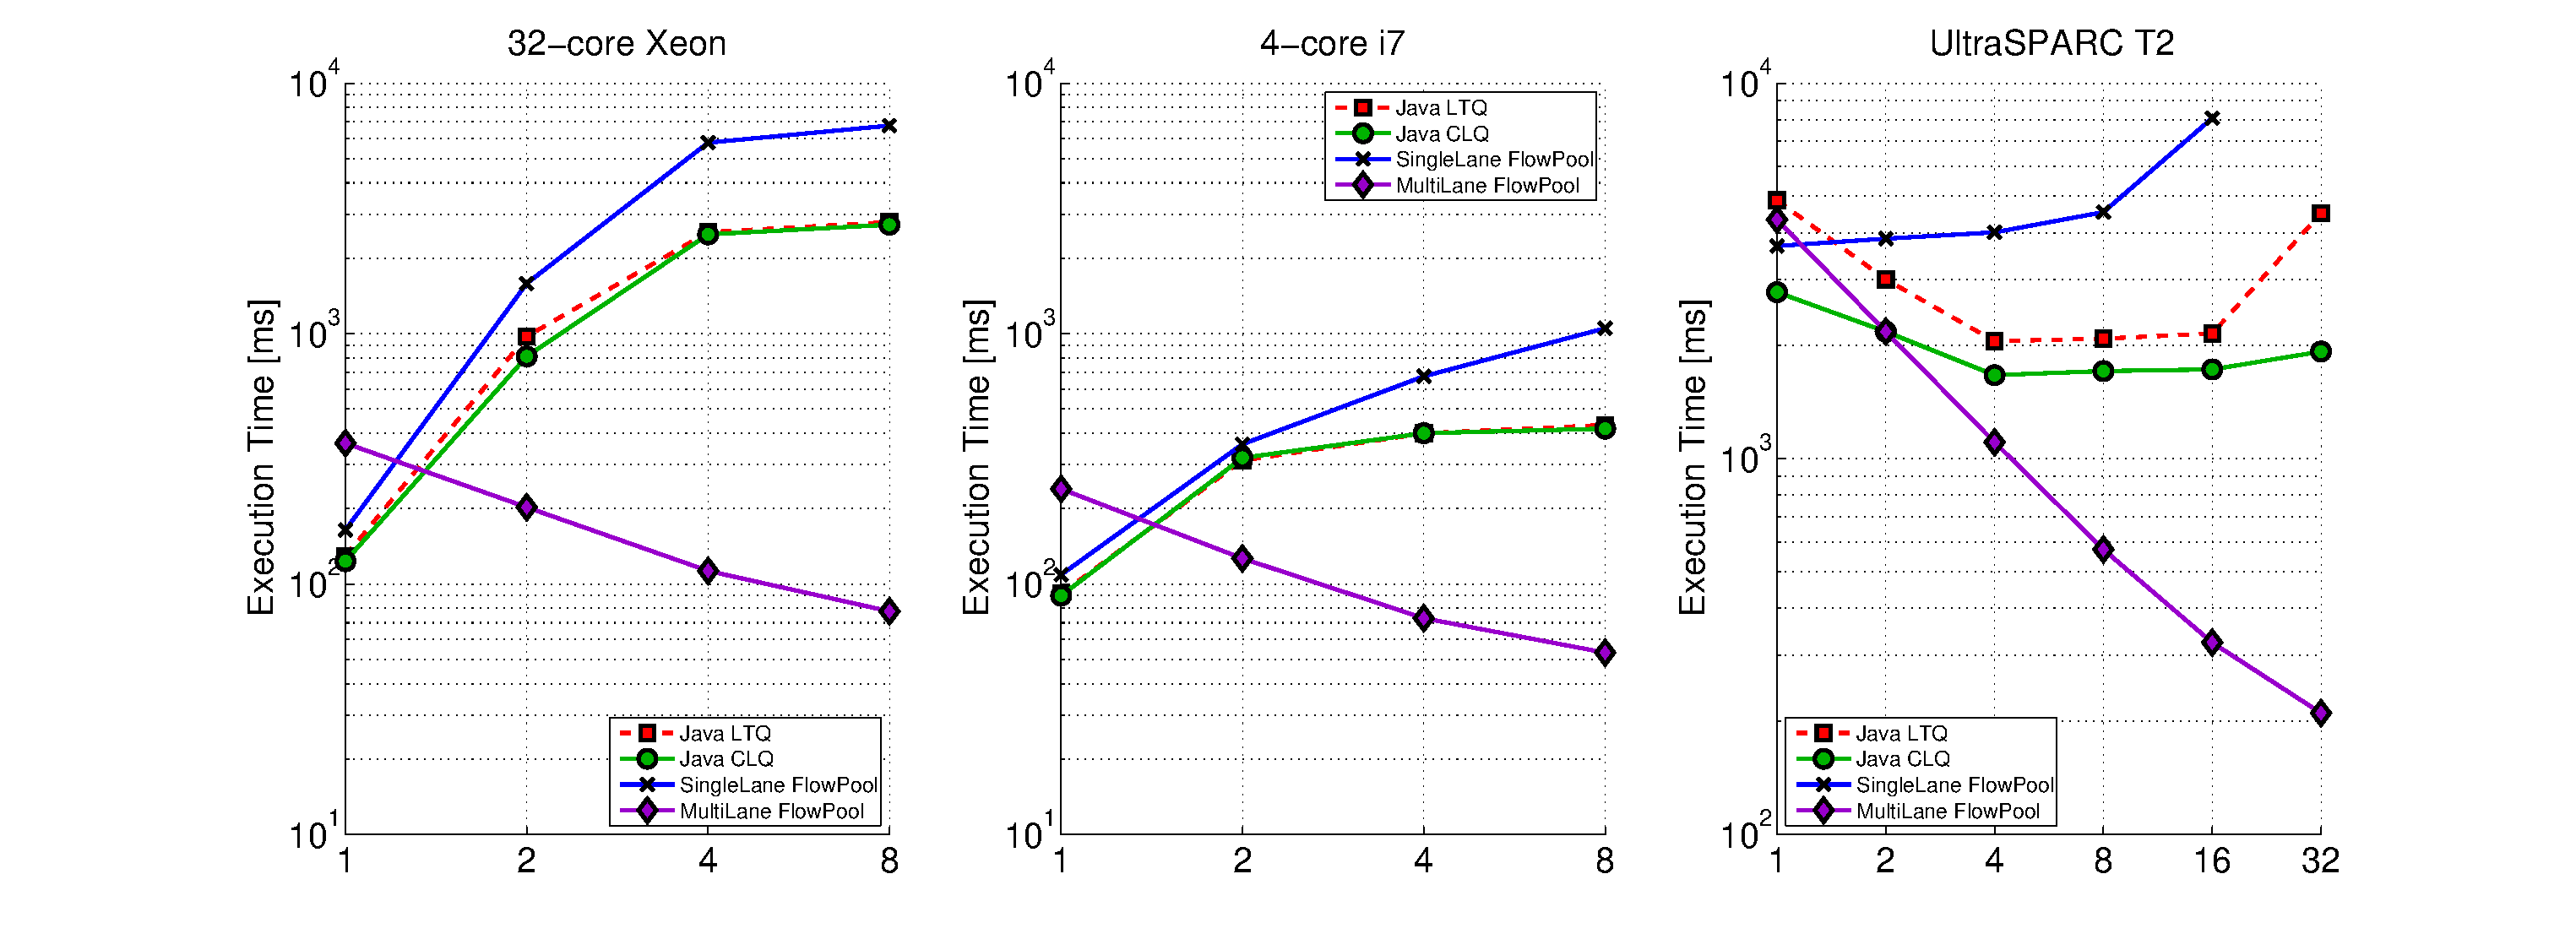
\includegraphics[trim = 35mm 0mm 36mm 0mm, clip, width=0.95\paperwidth]
      {../../benchmarks/pres_graphs/cpu-scaling-insert}
      \par
    \end{column}
  \end{columns}

\end{frame}

\begin{frame}
  \frametitle{Benchmarks}
  \framesubtitle{CPU-Scaling -- Reduce}

  %% Hack to use whole frame
  \begin{columns}[c]
    \begin{column}{\paperwidth}
      \centering
      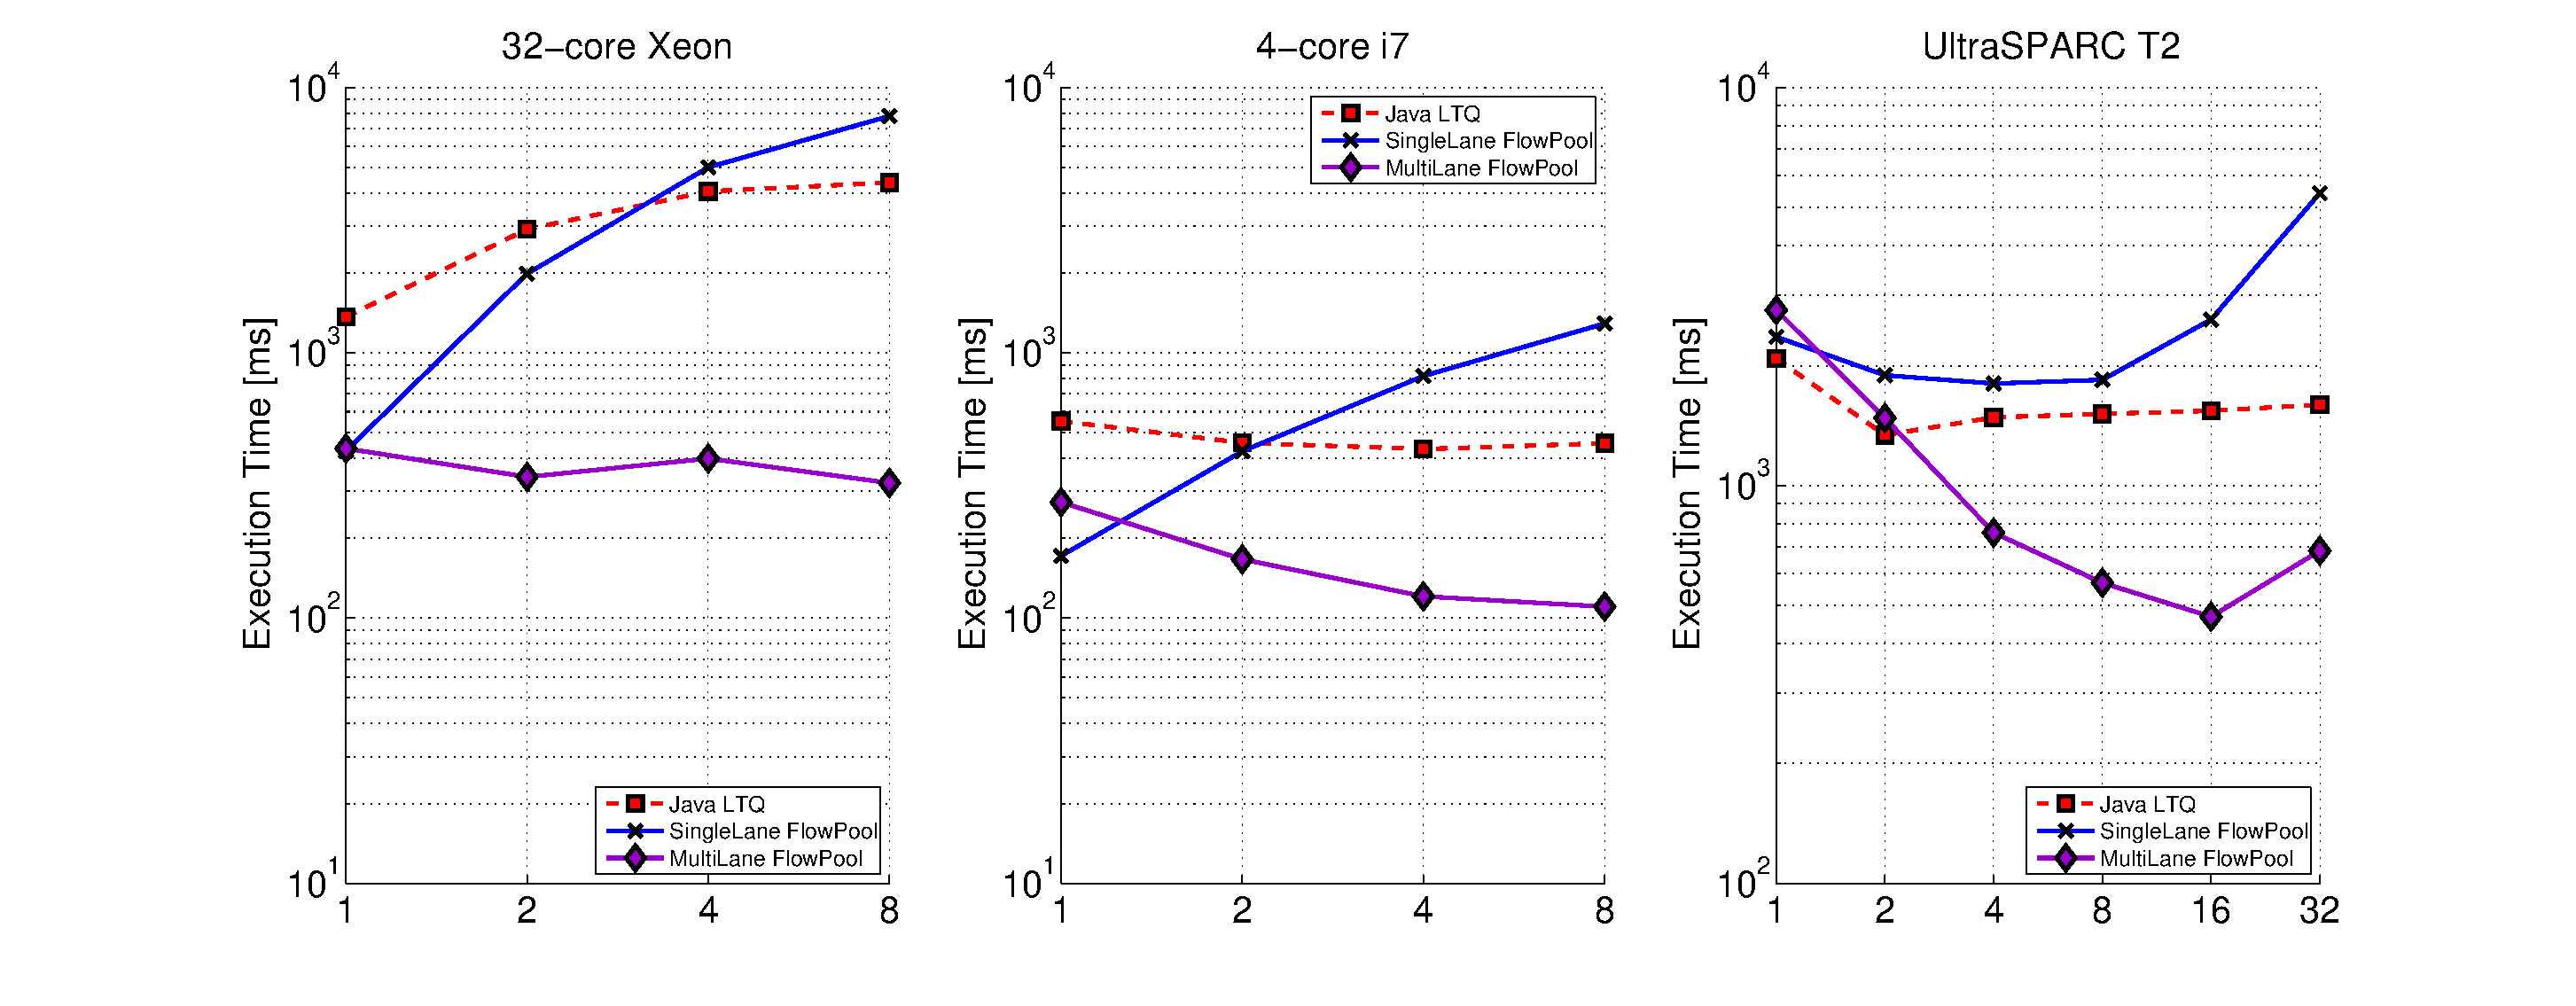
\includegraphics[trim = 35mm 0mm 36mm 0mm, clip, width=0.95\paperwidth]
      {../../benchmarks/pres_graphs/cpu-scaling-reduce}
      \par
    \end{column}
  \end{columns}

\end{frame}

\begin{frame}
  \frametitle{Benchmarks}
  \framesubtitle{CPU-Scaling -- Communication/Garbage Collection}

  %% Hack to use whole frame
  \begin{columns}[c]
    \begin{column}{\paperwidth}
      \centering
      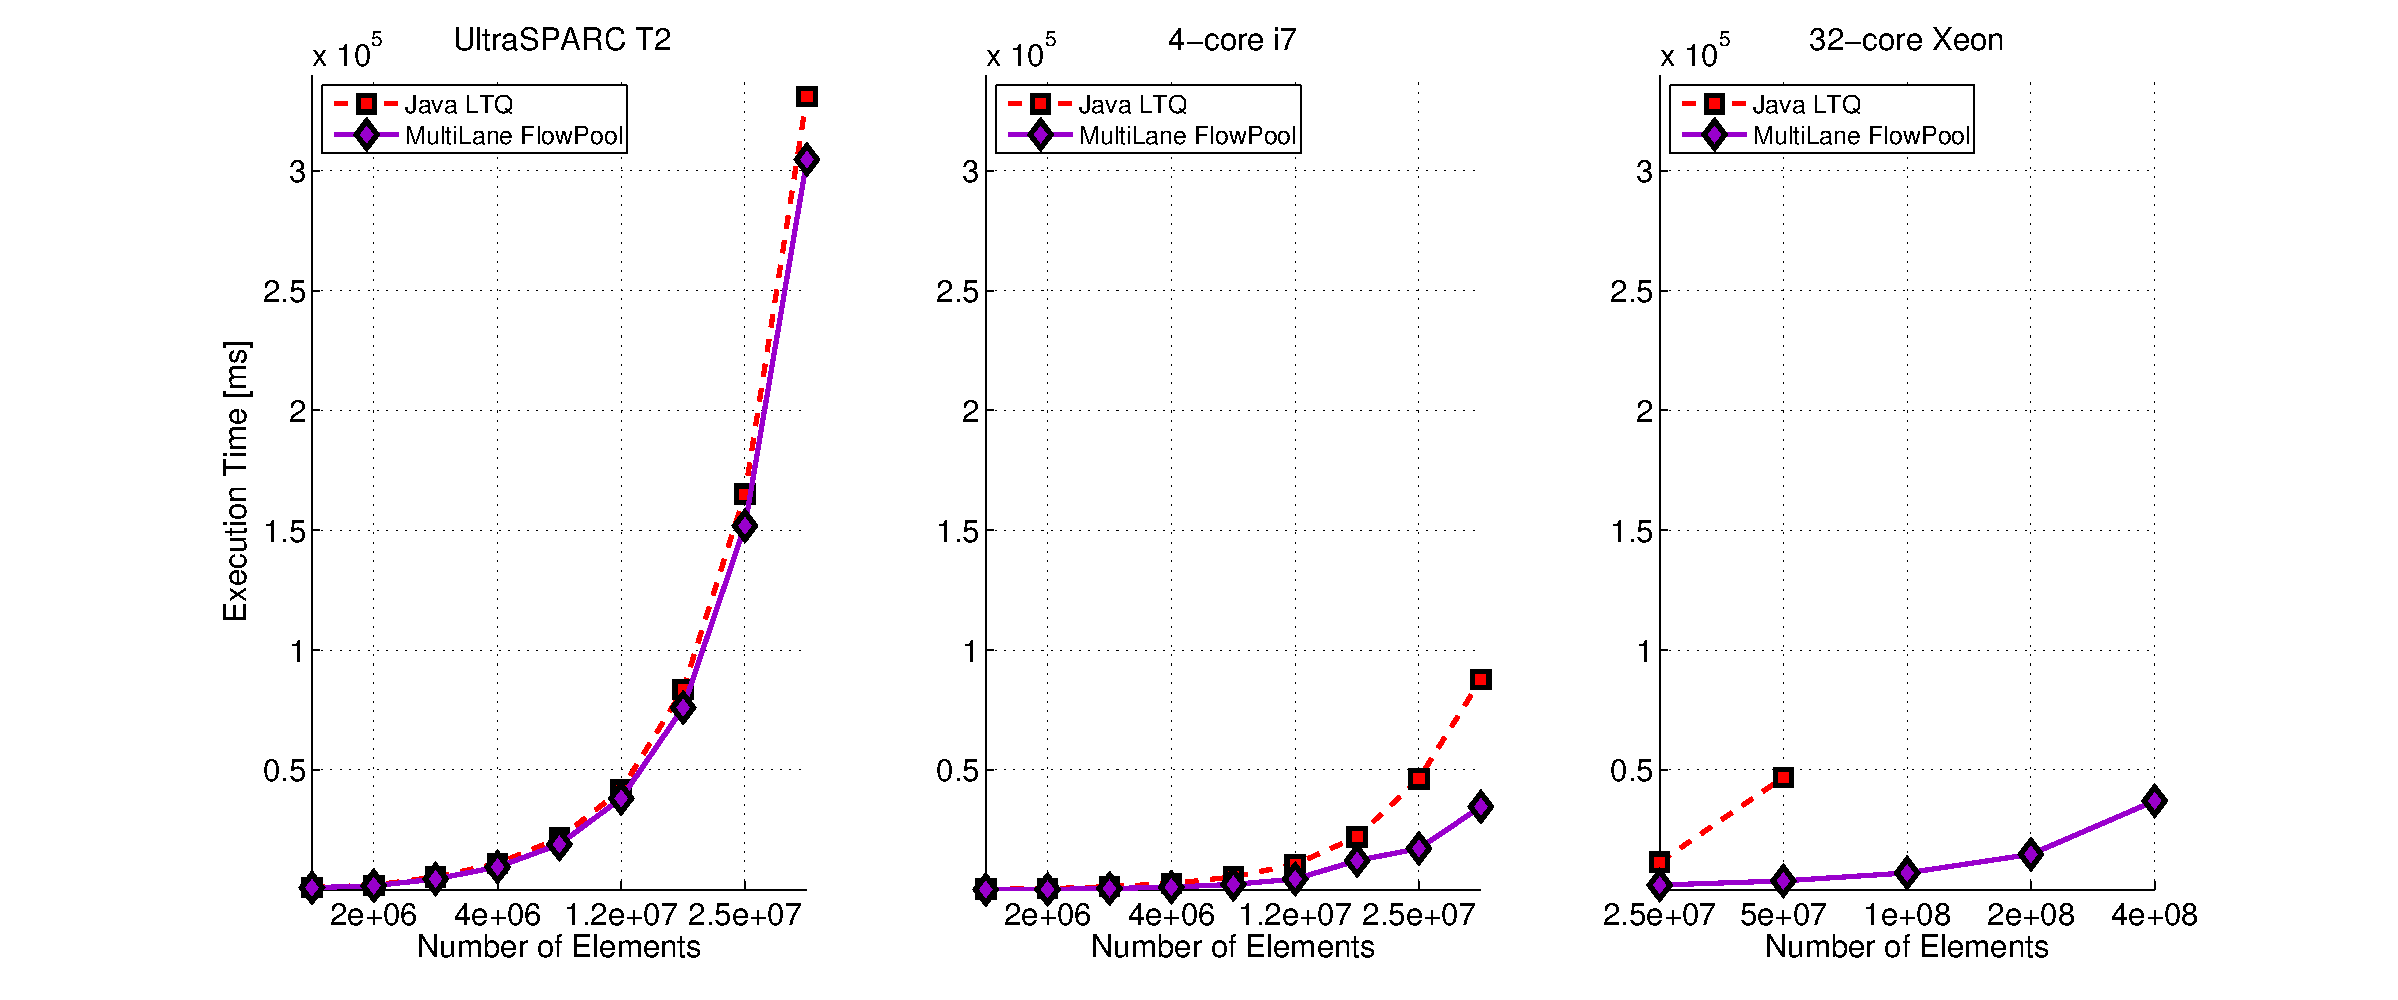
\includegraphics[trim = 35mm 0mm 32mm 0mm, clip, width=0.95\paperwidth]
      {../../benchmarks/pres_graphs/comm}
      \par
    \end{column}
  \end{columns}

\end{frame}

\section{Conclusion}

\begin{frame}
  \frametitle{Conclusion}

  {\Large FlowPools are \ldots}

  \pause
  \begin{block}{Basic Traits}
    \begin{itemize}
    \item Flow-Based Collection
    \item Asynchronous
    \item Deterministic
    \end{itemize}
  \end{block}
      
  \pause
  \begin{block}{Performance \& Scalability}
    \begin{itemize}
    \item Speed comparable to Java standard Queues
    \item Scalable
    \item Unneeded Elements GC'd
    \end{itemize}
  \end{block}

  \pause
  \begin{block}{¿Questions?}
  \end{block}

\end{frame}

\section{Appendix}

\begin{frame}
  \frametitle{Details about Benchmarks}

  \begin{columns}[t]
    \begin{column}{.5\textwidth}
      \begin{block}{Insert / Reduce}
        \begin{itemize}
        \item $5\cdot10^6$ elements
        \item 20 measurements
        \end{itemize}
      \end{block}

      \begin{block}{Communication / GC}
        \begin{itemize}
        \item Parallelization level: 1
        \item Measurements
          \begin{itemize}
          \item UltraSPARC T2: 2
          \item 4-core i7: 10
          \item 32-core Xeon: 3
          \end{itemize}
        \end{itemize}
      \end{block}

    \end{column}
    \begin{column}{.5\textwidth}
      \begin{block}{Java Command}
        \small\texttt{-Xmx2048m -Xms2048m -XX:+UseCondCardMark
          -verbose:gc -XX:+PrintGCDetails -server}.
      \end{block}
      \begin{block}{Java Version}
        \begin{itemize}
        \item Intel \small\texttt{
            1.7.0\_04-ea-b15\\
            HotSpot 64-Bit Server VM (build 23.0-b16, mixed mode)
          }
        \item SPARC \small\texttt{
            1.7.0\_03-b04\\
            HotSpot Server VM (build 22.1-b02, mixed mode)
          }
        \end{itemize}
      \end{block}
    \end{column}
  \end{columns}
    
\end{frame}

\begin{frame}
  \frametitle{Details about Benchmarks}

  \begin{block}{Architectures}
    \begin{itemize}
    \item octa-core 1.2GHz UltraSPARC T2 w/ 64 HW threads
    \item quad-core 3.4 GHz i7-2600 (w/ HT)
    \item 4x octa-core 2.27 GHz Intel Xeon x7560 (w/ HT)
    \end{itemize}
  \end{block}

\end{frame}

\begin{frame}
  \frametitle{Multi-Lane FlowPools}
  \framesubtitle{Basic Structure}
  \begin{center}
    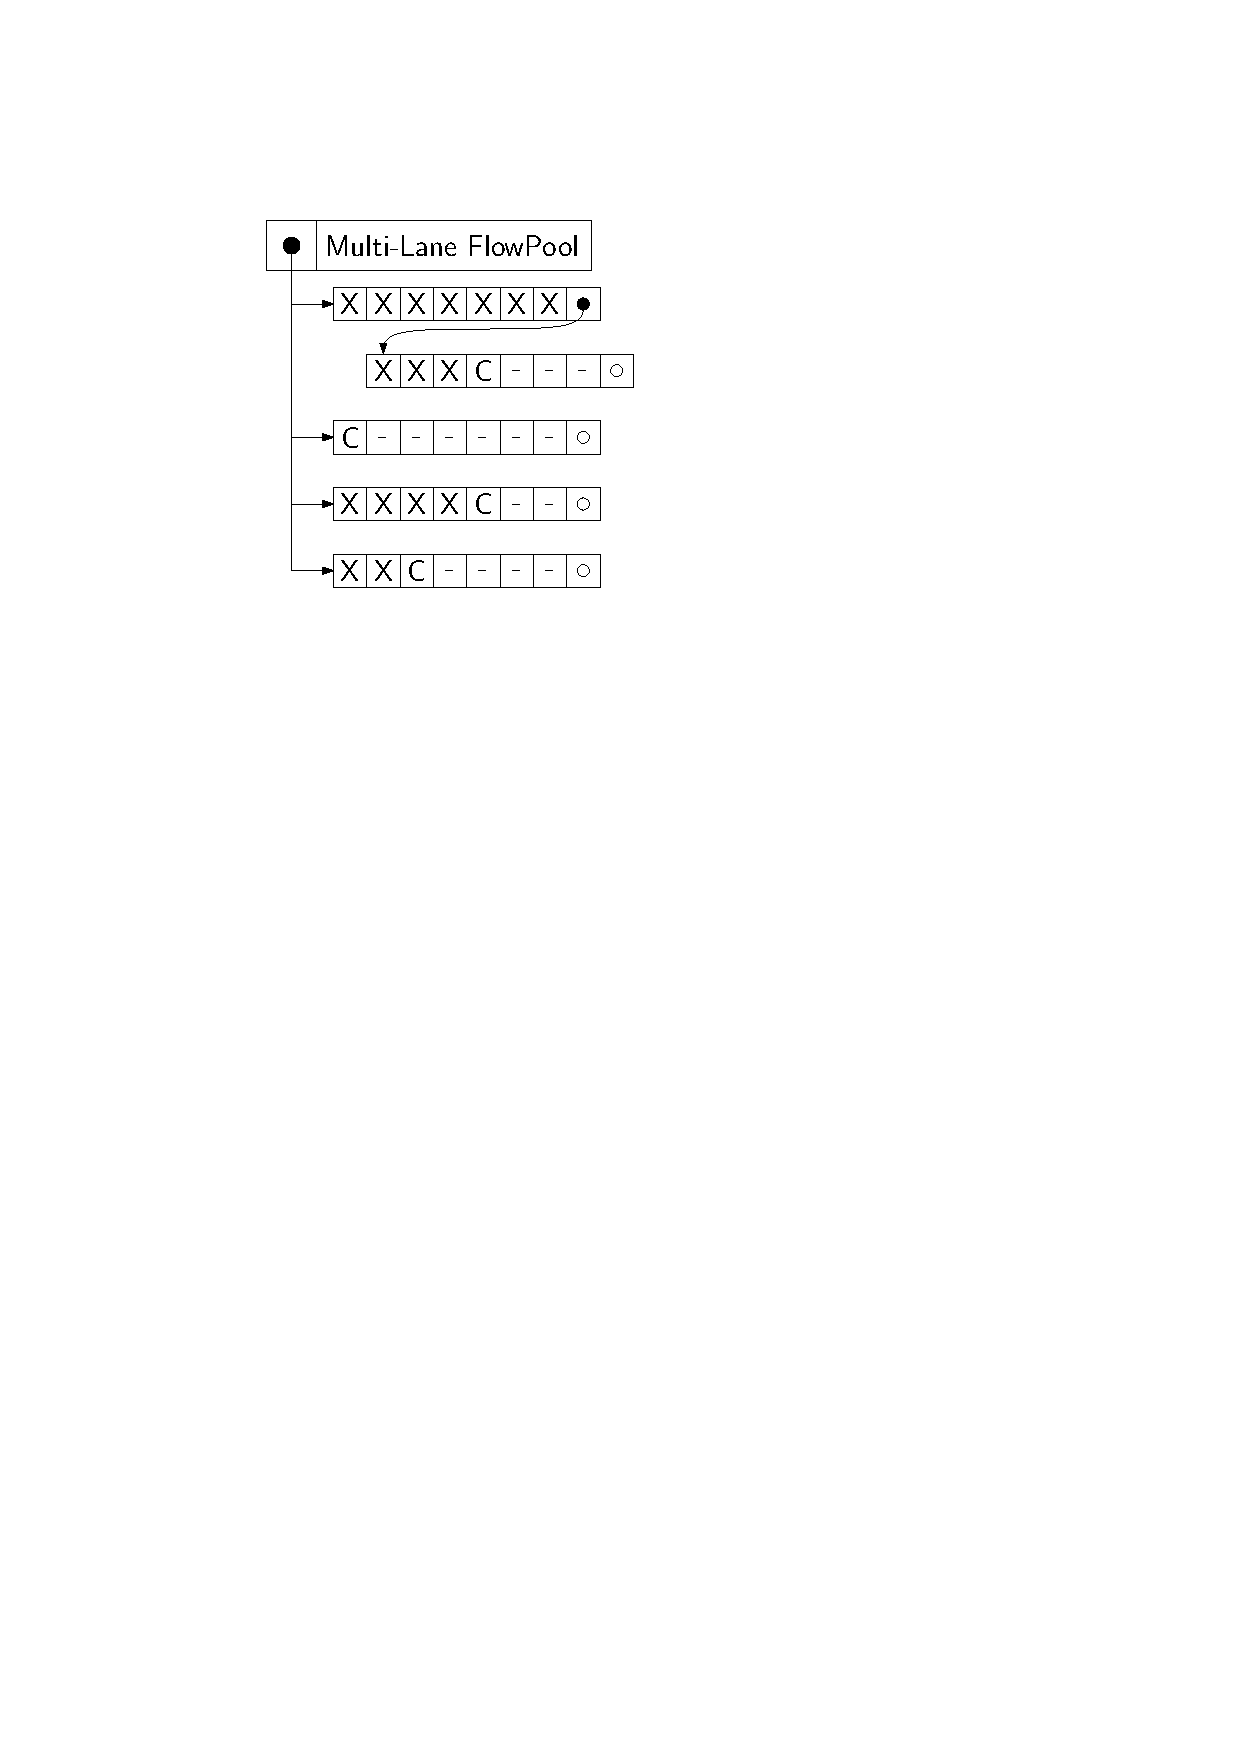
\includegraphics{figs/MLFP}
  \end{center}
\end{frame}

\begin{frame}
  \frametitle{Multi-Lane FlowPools}
  \framesubtitle{Seal \quad \texttt{\sF{seal}\sN(\sV n\sN:\;\sT{Int}\sN)}}

  \includegraphics<1>[page=1]{figs/MLFP_seal}
  \includegraphics<2>[page=2]{figs/MLFP_seal}
  \includegraphics<3>[page=3]{figs/MLFP_seal}
  \includegraphics<4>[page=4]{figs/MLFP_seal}
  \includegraphics<5>[page=5]{figs/MLFP_seal}
  \includegraphics<6>[page=6]{figs/MLFP_seal}
  \includegraphics<7>[page=7]{figs/MLFP_seal}
  \includegraphics<8>[page=8]{figs/MLFP_seal}

\end{frame}

\begin{frame}
  \frametitle{Multi-Lane FlowPools}
  \framesubtitle{Insert / Choice of Lane}

  \includegraphics<1>[page=1]{figs/MLFP_insert}
  \includegraphics<2>[page=2]{figs/MLFP_insert}
  \includegraphics<3>[page=3]{figs/MLFP_insert}
  \includegraphics<4>[page=4]{figs/MLFP_insert}
  \includegraphics<5>[page=5]{figs/MLFP_insert}
  \includegraphics<6>[page=6]{figs/MLFP_insert}
  \includegraphics<7>[page=7]{figs/MLFP_insert}
  \includegraphics<8>[page=8]{figs/MLFP_insert}
  \includegraphics<9>[page=9]{figs/MLFP_insert}
  \includegraphics<10>[page=10]{figs/MLFP_insert}
  \includegraphics<11>[page=11]{figs/MLFP_insert}

  \begin{textblock}{8}(8,2)
    \begin{enumerate}
    \item<1-> $L_{id} = T_{id} \bmod L_{tot}$
    \item<4-> $L_{id} = hash(T_{id} + C) \bmod L_{tot}$
    \item<7-> Exhaustive search
    \end{enumerate}
  \end{textblock}


\end{frame}

\begin{frame}
  \frametitle{Hash Function}

  \begin{block}{Byte-swap Hashing}
  \[ hash(x) = \text{rb}(x \cdot 9e3775cd_{16}) \cdot 9e3775cd_{16} \]
  \end{block}

\end{frame}

\begin{frame}
  \frametitle{Efficiency of Hashing}

  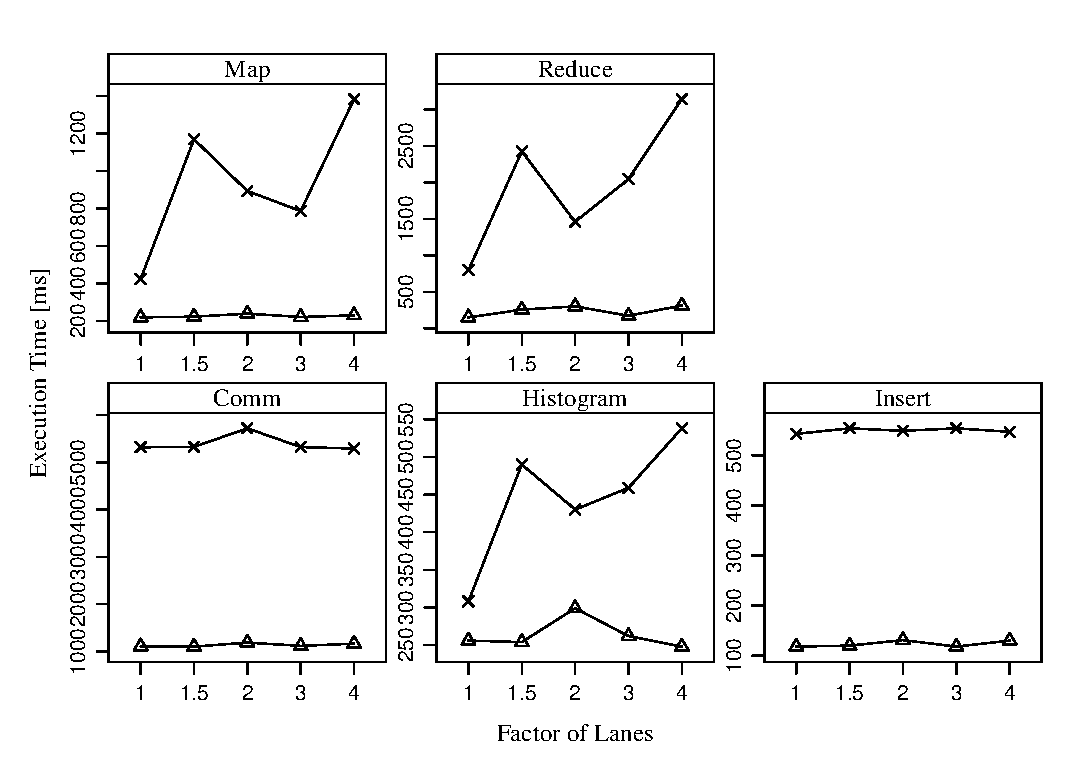
\includegraphics[width=\textwidth]{../../benchmarks/graphs/lanef-scaling}\\
  $\times$ UltraSPARC T2, $\triangle$ 4-core i7

\end{frame}

\end{document}

%%% Local Variables: 
%%% mode: latex
%%% TeX-master: t
%%% End: 
